\section{}
\[
H(s)=\frac{100\,(s+1)}{s^2+20s+100}=\frac{100\,(s+1)}{(s+10)^2}\,.
\]
\subsection{Bode-Diagramm}
\begin{center}
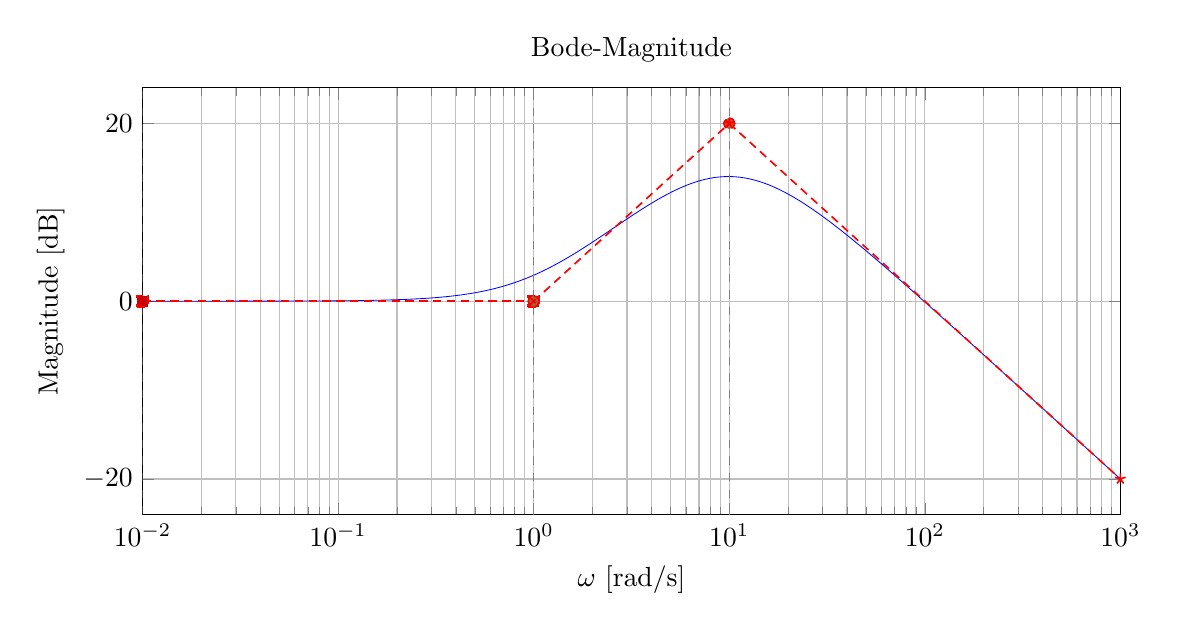
\begin{tikzpicture}
\begin{semilogxaxis}[
  width=14cm,height=7cm,
  xmin=1e-2,xmax=1e3,
  xlabel={$\omega$ [rad/s]},
  ylabel={Magnitude [dB]},
  grid=both,
  ytick distance=20,
  title={Bode-Magnitude}
]
\addplot[
  domain=1e-2:1e3,
  samples=600,
  mark=none,
  line width=0.3pt,
  blue
] {40 + 20*ln(sqrt(1 + x^2))/ln(10) - 40*ln(sqrt(100 + x^2))/ln(10)};
\addplot+[domain=1e-2:1,samples=2,dashed,dash pattern=on 3pt off 2pt,line width=0.6pt,red] {0};
\addplot+[domain=1:1e1,samples=2,dashed,dash pattern=on 3pt off 2pt,line width=0.6pt,red] {20*ln(x)/ln(10)};
\addplot+[domain=1e1:1e3,samples=2,dashed,dash pattern=on 3pt off 2pt,line width=0.6pt,red] {20 - 20*ln(x/10)/ln(10)};
\draw[gray,dashed] (rel axis cs:0,0) -- (rel axis cs:0,1);
\draw[gray,dashed] (axis cs:1,\pgfkeysvalueof{/pgfplots/ymin}) -- (axis cs:1,\pgfkeysvalueof{/pgfplots/ymax});
\draw[gray,dashed] (axis cs:10,\pgfkeysvalueof{/pgfplots/ymin}) -- (axis cs:10,\pgfkeysvalueof{/pgfplots/ymax});
\node[gray,anchor=south east] at (axis cs:1,\pgfkeysvalueof{/pgfplots/ymax}) {\scriptsize Nullstelle $\omega_z=1$};
\node[gray,anchor=south east] at (axis cs:10,\pgfkeysvalueof{/pgfplots/ymax}) {\scriptsize Pol $\omega_p=10$ (doppelt)};
\end{semilogxaxis}
\end{tikzpicture}
\vspace{6mm}
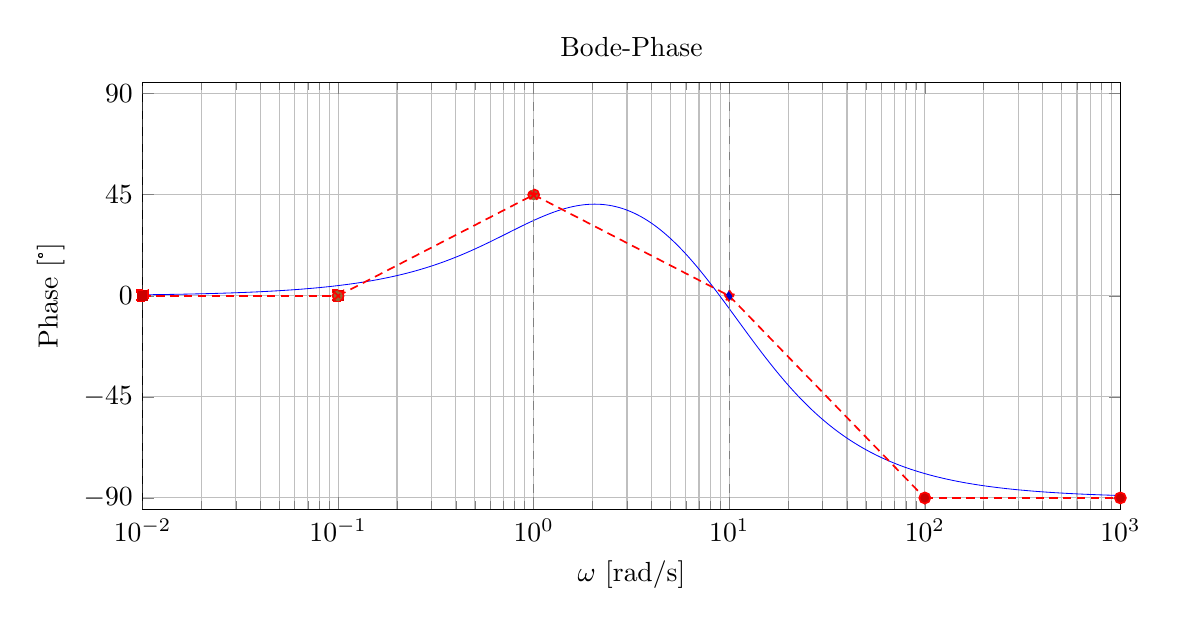
\begin{tikzpicture}
\begin{semilogxaxis}[
  width=14cm,height=7cm,
  xmin=1e-2,xmax=1e3,
  ymin=-95,ymax=95,
  ytick distance=45,
  xlabel={$\omega$ [rad/s]},
  ylabel={Phase [°]},
  grid=both,
  title={Bode-Phase}
]
\addplot[
  domain=1e-2:1e3,
  samples=600,
  mark=none,
  line width=0.3pt,
  blue
] {atan(x) - 2*atan(x/10)};
\addplot+[domain=1e-2:1e-1,samples=2,dashed,dash pattern=on 3pt off 2pt,line width=0.6pt,red] {0};
\addplot+[domain=1e-1:1e0,samples=2,dashed,dash pattern=on 3pt off 2pt,line width=0.6pt,red] {45 + 45*ln(x)/ln(10)};
\addplot+[domain=1e0:1e1,samples=2,dashed,dash pattern=on 3pt off 2pt,line width=0.6pt,red] {45 - 45*ln(x)/ln(10)};
\addplot+[domain=1e1:1e2,samples=2,dashed,dash pattern=on 3pt off 2pt,line width=0.6pt,red] {-90*ln(x/10)/ln(10)};
\addplot+[domain=1e2:1e3,samples=2,dashed,dash pattern=on 3pt off 2pt,line width=0.6pt,red] {-90};
\draw[gray,dashed] (rel axis cs:0,0) -- (rel axis cs:0,1);
\draw[gray,dashed] (axis cs:1,\pgfkeysvalueof{/pgfplots/ymin}) -- (axis cs:1,\pgfkeysvalueof{/pgfplots/ymax});
\draw[gray,dashed] (axis cs:10,\pgfkeysvalueof{/pgfplots/ymin}) -- (axis cs:10,\pgfkeysvalueof{/pgfplots/ymax});
\node[gray,anchor=south east] at (axis cs:1,\pgfkeysvalueof{/pgfplots/ymax}) {\scriptsize Nullstelle $\omega_z=1$};
\node[gray,anchor=south east] at (axis cs:10,\pgfkeysvalueof{/pgfplots/ymax}) {\scriptsize Pol $\omega_p=10$ (doppelt)};
\end{semilogxaxis}
\end{tikzpicture}
\end{center}
\newpage
\subsection{Erklärung}
\vspace{5mm}
\begin{description}[leftmargin=1.2em,labelsep=.6em,font=\bfseries]
\item[Schritt 1] Faktorisierung: $s^2+20s+100=(s+10)^2\Rightarrow H(s)=100\,\dfrac{s+1}{(s+10)^2}$. DC-Wert $H(0)=1\Rightarrow |H|_{\mathrm{DC}}=0\,\mathrm{dB}$; Anfangssteigung $0\,\mathrm{dB/dec}$, Startphase $\approx0^\circ$.
\item[Schritt 2] Nullstelle bei $\omega_z=1\,\mathrm{rad/s}$: ab $\omega=1$ steigt die Magnitude mit $+20\,\mathrm{dB/dec}$ (rote Gerade $20\log_{10}\omega$). Exakt bei $\omega=1$: $|H(\j1)|\approx\frac{100\sqrt{2}}{101}\Rightarrow |H|_{\mathrm{dB}}\approx+3\,\mathrm{dB}$ über der Geraden. Phasenbeitrag der LHP-Nullstelle: Übergang $0^\circ\to+90^\circ$ über $\omega\in[0.1,10]$ (Geradennäherung: $45^\circ+45\log_{10}\omega$).
\item[Schritt 3] Doppelpol bei $\omega_p=10\,\mathrm{rad/s}$: ab $\omega=10$ zusätzliche Steigungsänderung um $-40\,\mathrm{dB/dec}$; Netto-Slope für $\omega\gg10$ ist $-20\,\mathrm{dB/dec}$ (asymptotisch $|H|\sim100\,\omega/\omega^2=100/\omega$). Am Eckpunkt $\omega=10$ liegt die exakte Magnitude bei $\approx14.0\,\mathrm{dB}$, d.\,h.\ etwa $-6\,\mathrm{dB}$ unter der Mittellinie. Phasenabfall der beiden Pole gesamt $180^\circ$ über $\omega\in[1,100]$; Geradennäherung: zunächst $45^\circ-45\log_{10}\omega$ für $\omega\in[1,10]$ (netto zurück Richtung $0^\circ$), danach $-90\log_{10}(\omega/10)$ für $\omega\in[10,100]$ (netto bis $-90^\circ$).
\end{description}

\vspace{0.5cm}
\medskip
\noindent\textbf{Stückweise Näherung}
\[
|H(\j\omega)|_{\mathrm{dB}}\approx
\begin{cases}
0,& \omega\ll1,\\[4pt]
20\log_{10}\omega,& 1\ll\omega\ll10,\\[4pt]
20-20\log_{10}(\omega/10),& \omega\gg10,
\end{cases}
\qquad
\]
\newpage